%%%%%%%%%%%%%%%%%%%%%%%%%%%%%%%%%%%%%%%%%%%%%%%%%%%%%%%%%%%%%%%%%%%%%%%%%%%%%% 
\newpage
\section {RMC spectrum and $\kmax$ determination}

Measured RMC photon spectra on nuclei can be successfully described within 
the closure approximation, which predicts the RMC photon spectrum depending
on just one parameter - the photon spectrum endpoint:
$$
    \frac{dN}{dE} ~=~ \frac{e^2}{\pi} \frac{\kmax^2}{ m_{\mu}^2} (1 - \alpha) (1-x+2x^2)x(1-x)^2
$$
where E is the photon energy, $\kmax$ is the energy spectrum endpoint, $\rm \alpha = (N-Z)/A$,
and $x = E/\kmax$ \cite{Christillin_1980}.

Values of $\kmax$ for different nuclei are not predicted, but determined from the fits
to experimental data. Typically, fits return $\kmax$ values significantly lower than
the kinematically allowed limits. 

Internal conversions from RMC will also contribute to the measured spectrum, but as the virtual
photon energy distribution should be the same as the real RMC photon energy
distribution, and since the energy sharing between the positron and electron
is similar to that of photon conversions, this contribution should be captured by
fitting the spectrum normalization.

We determine the value of the $\kmax$ parameter by fitting the SINDRUM-II positron spectrum
with a closure approximation spectrum convolved with the resolution $\sigma_P = 2$ MeV/c
and the efficiency determined from the fit to the electron spectrum
(see Figure ~\ref{fig:ana_step1_efficiency}) and vary the value of $\kmax$.
Results of the fit are shown in Figure ~\ref{fig:ana_step2_fit_kmax}, the best fit
corresponds to $\kmax = 88.0 \pm 0.6$ MeV.
%
With the energy losses taken into account, the value becomes  $\kmax = 88.6 \pm 0.6$ MeV.
The maximal photon energy allowed kinematically in a 
$$
\rm \mu^- + \Au{197}(GS) \rightarrow \nu +\gamma + ^{197}Pt(GS)
$$
transition is $E_{max} = 94.3$ MeV, which is several MeV higher.

\vspace{0.1in}
\begin{tikzpicture}
  \node[anchor=south west,inner sep=0] at (0,0.) {
    % \node[shift={(0 cm,0.cm)},inner sep=0,rotate={90}] at (0,0) {}
    \makebox[\textwidth][c] {
      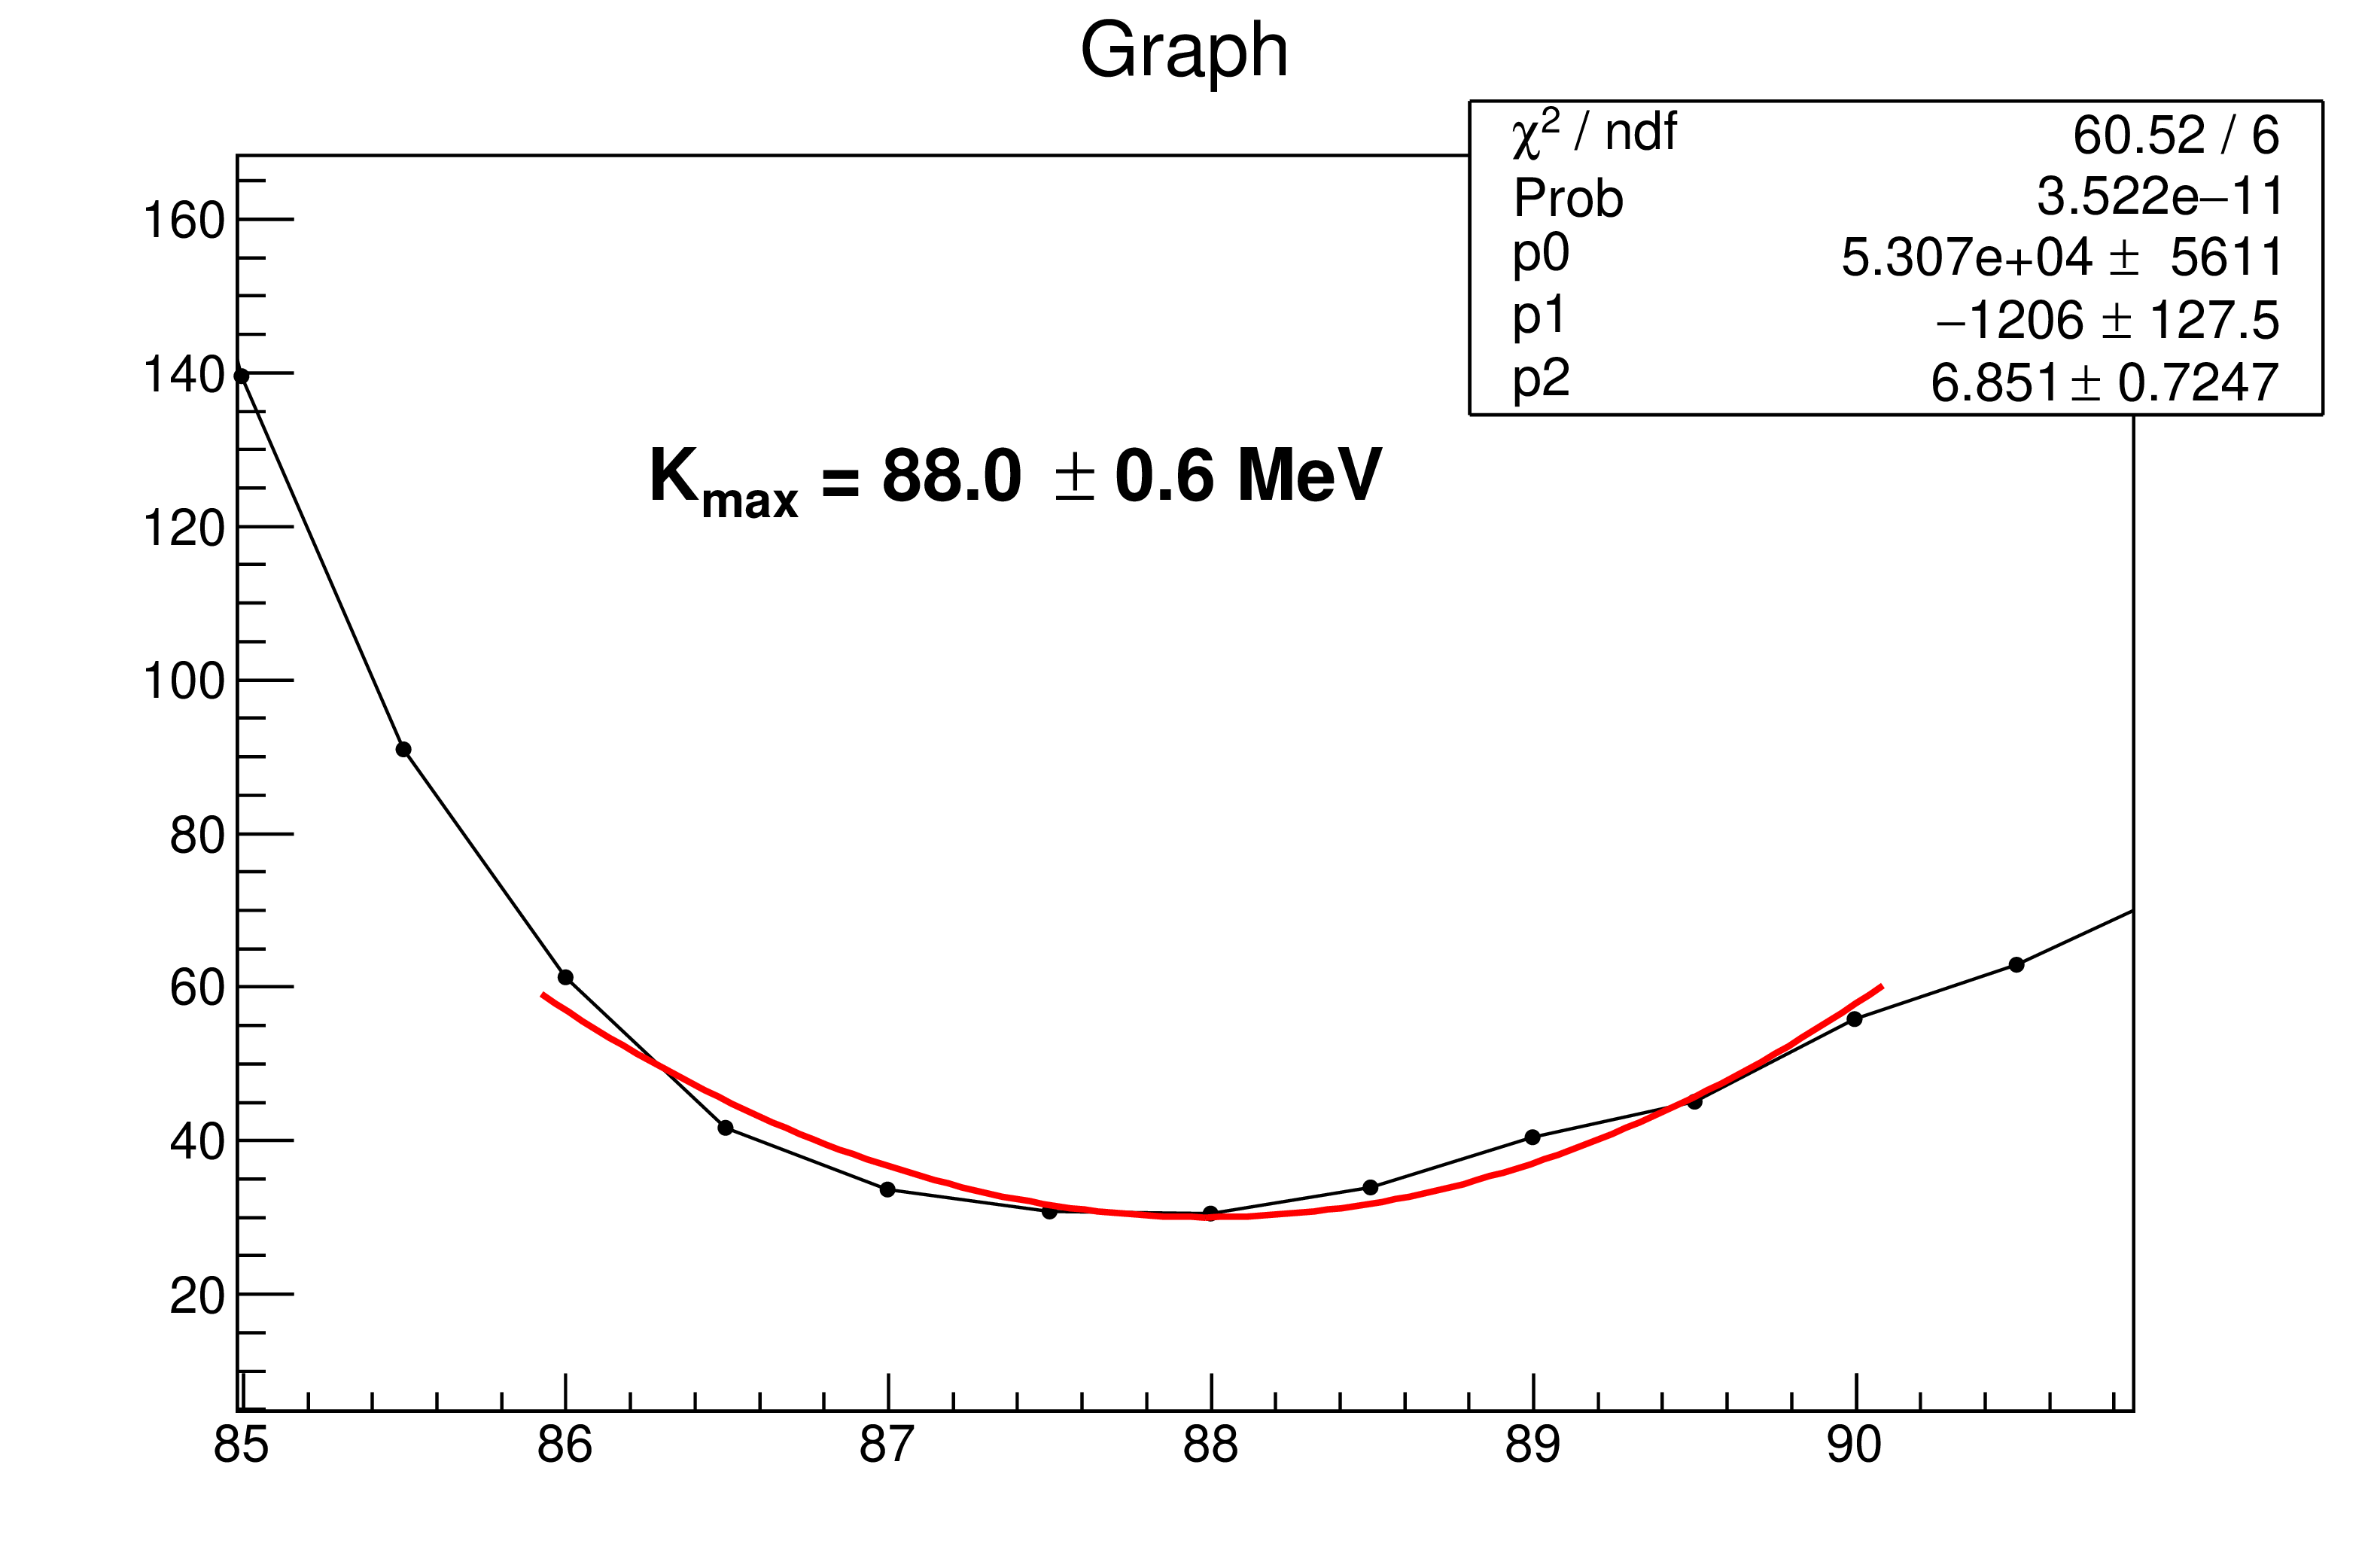
\includegraphics[width=1.0\textwidth, trim = 180 0 50 125,clip]{figures/png/ana_step2_fit_kmax}
    }
  };
  % \node [text width=6cm, scale=0.8] at (4.5,6.4) {mu2e-18894 by Kevin Lynch and Jim Popp};
\end{tikzpicture}
\captionof{figure} {
  \label{fig:ana_step2_fit_kmax}
  $\chi^2$ of the SINDRUM-II positron spectrum fit with the posiron momentum distribution
  derived from the RMC closure approximation spectrum convolved with the detector response. 
  Used in the fit are events with p < 88 MeV/c.
}
\vspace{0.1in}


%% Local Variables:
%%% mode: latex
%%% TeX-master: t
%%% End:
